\chapter{绪论}

\section{研究背景}

\begin{wrapfigure}{r}{0.5\linewidth}
    \centering
        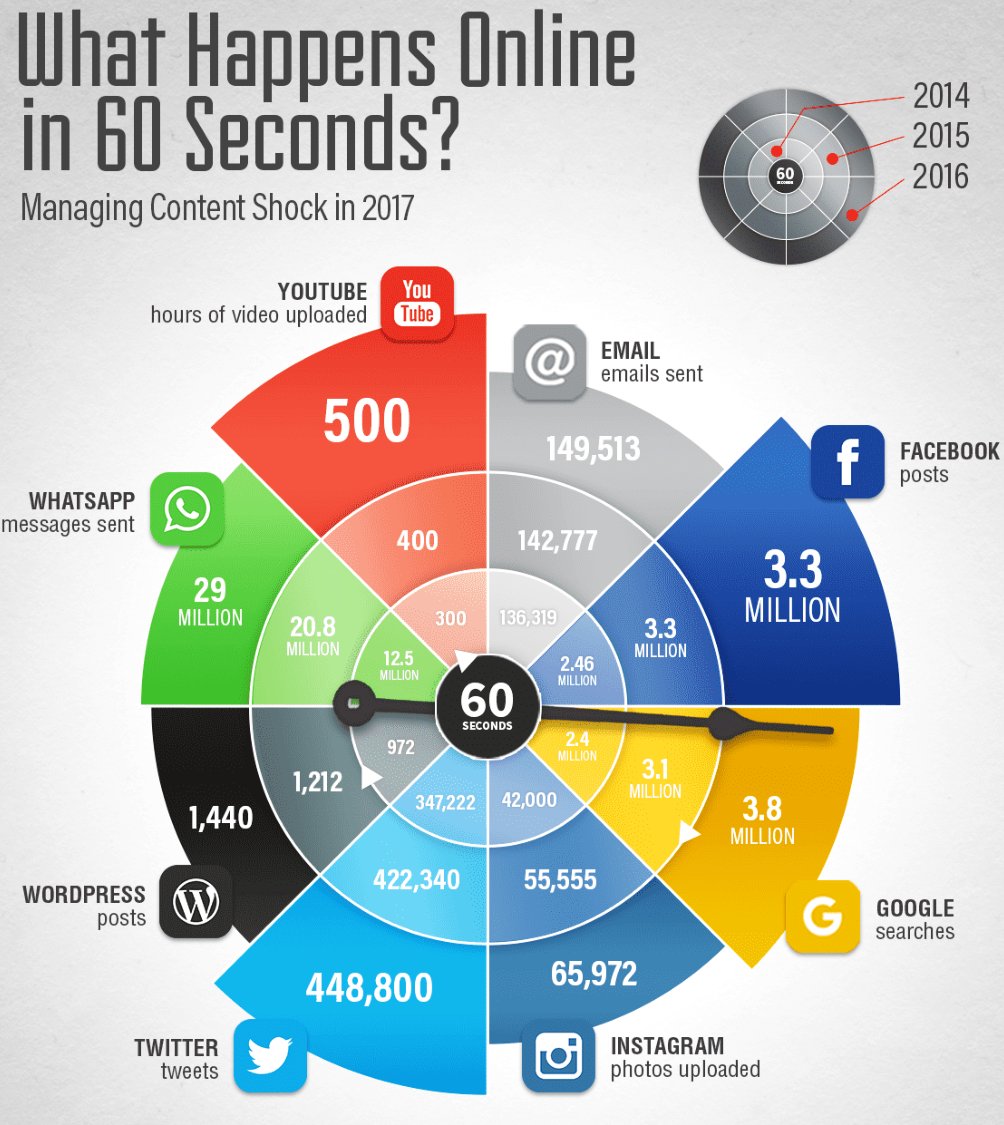
\includegraphics[width=0.95\linewidth]{chapter1/res/media_statistics.pdf}
    \captionof{figure}{大数据时代下图像、视频等媒体数据呈现“爆炸式”增长}
    \label{ch1:fig:media_statistics}
\end{wrapfigure}

视觉是人类感知外界客观世界的主要信息来源,而计算机视觉技术旨在让机器能够像人类一样准确地感知和理解物理世界。计算机视觉技术的发展和进步,是众多人机交互技术的基石,也是人类社会迈向真正人工智能时代至关重要的一步。目前,随着互联网技术、社交媒体技术的快速发展以及数字媒体设备、便携式设备的全面普及,图像、动态图、视频等多种形式的视觉媒体数据都呈现“爆炸式”增长。如图~\ref{ch1:fig:media_statistics}所示\footnote{图片来源:https://www.smartinsights.com/internet-marketing-statistics/happens-online-60-seconds/},截止到2016年,视频分享网站YouTube每分钟上传约500小时视频数据,图像分享社区Instagram每分钟上传约65972张图像数据。面对日益增长的海量视觉媒体数据,利用计算机视觉技术对其进行感知和理解,从而实现对海量视觉媒体数据的快速利用,对便利人们的日常生活、推动人类社会的进步都有着十分重大的意义和应用价值。

与此同时,如图~\ref{ch1:fig:datasets_examples}所示,随着近年来众多大规模图像和视频数据集的出现~\cite{lin2014microsoft,russakovsky2015imagenet,krishna2017visual,karpathy2014large,miech2019howto100m},基于深度学习~\cite{lecun2015deep,krizhevsky2012imagenet}的计算机视觉技术取得了重大突破,在多个视觉任务中达到甚至超过人类的表现。例如,在大规模图像分类数据集ImageNet上,最新的计算机视觉模型~\cite{xie2019self}在Top-1类别的分类准确率高达88.4\%、在Top-5类别的分类准确率高达98.7\%,而人类在Top-5类别的分类准确率只有94.9\%~\cite{russakovsky2015imagenet}。然而,对于复杂视觉场景的感知和理解,目前的计算机模型的表现与人类的表现还相差甚远,远远没有达到大规模普及和落地应用的水平。这主要原因来自于复杂视觉场景中通常包含大量的物体以及物体间的交互,同时物体间还存在各种遮挡、尺度不同等问题,这些都大大增加了视觉场景感知和理解的难度。另一方面,日常生活中的视觉媒体数据通常都是包含复杂的视觉场景内容。为了充分地利用这些海量的视觉媒体数据,复杂视觉场景的感知和理解已逐渐成为近年来计算机视觉领域的一个研究热点。

\begin{figure}[t]
    \centering
        \includegraphics[width=0.95\linewidth]{chapter1/res/datasets_examples.pdf}
    \caption{众多大规模图像和视频数据集推动计算机视觉技术的发展}
    \label{ch1:fig:datasets_examples}
\end{figure}

对于复杂视觉场景的感知和理解,具体来说,主要包含四个不同的层次:1)对场景内单个物体进行识别(\textbf{物体识别});2)对场景内所有物体以及物体之间的视觉关系进行识别(\textbf{场景识别});3)对整个视觉场景的内容进行理解(\textbf{场景理解});4)对整个视觉场景在理解的基础上进行知识推理(\textbf{场景推理})。本文将针对这四个不同层次的视觉场景感知和理解,逐步地对复杂视觉场景中视觉内容的识别、检测和推理进行研究。如图~\ref{ch1:fig:scene_understanding}所示,本文的关键技术线路主要物体分类(零样本物体分类)、场景图生成、视觉描述生成、视觉检索和视觉问答等具体研究任务:

\begin{figure}[t]
    \centering
        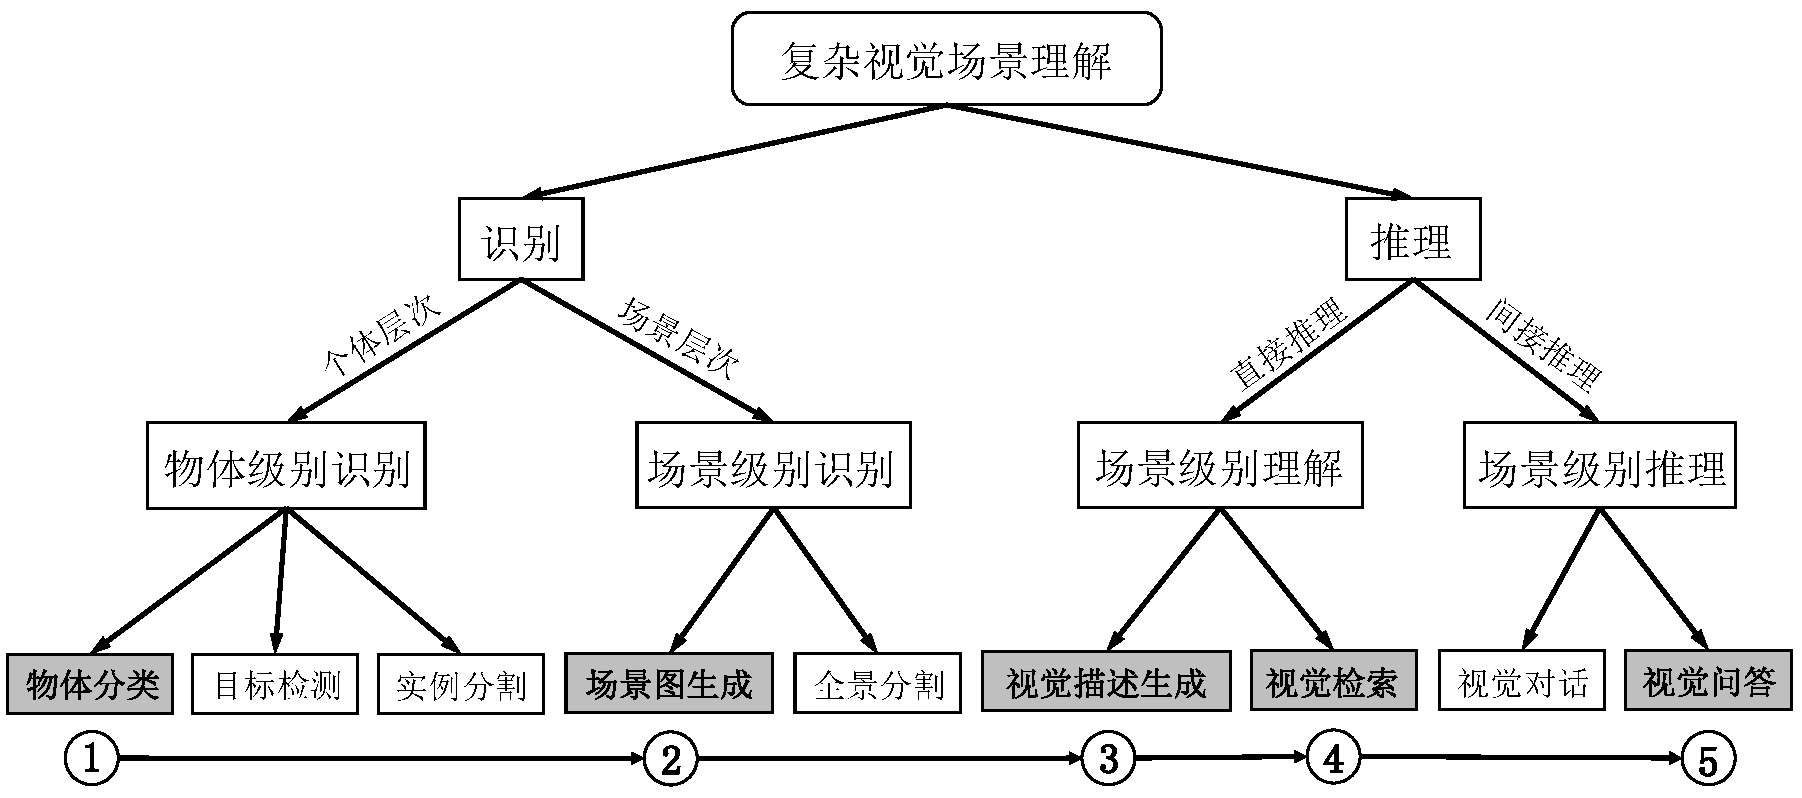
\includegraphics[width=0.95\linewidth]{chapter1/res/scene_understanding.pdf}
    \centering
    \caption{复杂视觉场景中视觉内容的识别、检测和推理的关键技术路线}
    \label{ch1:fig:scene_understanding}
\end{figure}

1)\textbf{物体识别}:视觉场景感知和理解的首要步骤就是对场景内包含的物体进行个体层次的识别。作为计算机视觉领域中一个最基本的问题,个体层次的物体识别结果将直接影响后续对整个视觉场景进行场景层次的识别、理解和推理。根据识别的粒度,物体识别通常包含物体分类、目标检测、实例分割等多种具体的视觉任务。其中物体分类任务~\cite{russakovsky2015imagenet,krizhevsky2012imagenet,simonyan2015very,szegedy2015going,he2016deep,xie2017aggregated,hu2018squeeze}只是对物体进行多类别分类,而目标检测任务~\cite{ren2015faster,liu2016ssd,redmon2016you}和实例分割任务~\cite{he2017mask}需要在物体分类的基础上,同时对物体的大致边框位置或精确像素位置进行定位。随着卷积神经网络的发展,在理想实验条件下,当每个类别的训练样本足够充足时,物体识别已经可以达到较高的准确率。然而,在日常生活中,所有类别的样本数量常常呈现“长尾分布”(long-tail distribution),即大量的类别往往缺乏足够的训练样本。例如,在大规模图像分类数据集ImageNet中,除最常见的1000类图像以外,在剩余的21814个类别中,有296个类别只有一张训练样本图像~\cite{russakovsky2015imagenet}。为了提升物体识别模型的通用性和鲁棒性,更加接近实际应用场景的少样本学习(Few-Shot Learning, FSL)~\cite{fei2006one}或零样本学习(Zero-Shot Learning, ZSL)~\cite{lampert2009learning}逐渐成为近年来的研究热点。然而,目前的零样本物体分类模型普遍存在语义丢失的问题(semantic loss),这将大大限制模型的迁移能力。本文将聚焦于零样本物体分类任务,研究如何减少模型的语义丢失,提升模型的通用性和鲁棒性。

2)\textbf{场景识别}:视觉场景的组成元素除了大量的规则物体(object)外,还包括不规则物体(stuff),以及物体之间的视觉关系(visual relationship)等。因此,对整个视觉场景进行感知和理解的第二步就需要对场景中所有的不规则物体(全景分割~\cite{kirillov2019panoptic})和视觉关系(场景图生成~\cite{johnson2015image})进行识别。尤其对于复杂场景来说,丰富的视觉关系通常“隐式地”包含场景内所有物体之间的内在联系。充分利用视觉关系不仅可以帮助提升单个物体的识别,同时可以将非结构化的视觉场景内容转换成结构化的场景图(scene graph)。这些场景图可以看成视觉场景内容的一种抽象知识表达,能够辅助更高语义层级的场景理解和推理。然而,目前的场景图生成模型主要都集中于研究如何更加有效地编码物体间的内在联系,并使用所有物体和视觉关系分类的交叉熵之和作为优化目标。这个优化目标忽略了不同物体对整体场景图质量的贡献差异,大大降低了训练梯度的优化效率。本文将聚焦于图像场景图生成任务,研究如何设计更加合理的优化目标,提升场景图生成质量以及提供更加有效的训练梯度。

3)\textbf{场景理解}:在对整个视觉场景中所有的组成元素都完成识别之后,就可以开始对场景内容进行理解和推理。就场景理解而言,如何判断一个计算机模型对视觉场景的理解程度,通常缺乏统一的衡量方式和标准的评价指标。随着自然语言处理领域的发展,众多视觉和文本融合的多模态任务开始被当作视觉场景理解的代理任务:如视觉描述生成~\cite{vinyals2015show}、视觉检索~\cite{gao2017tall}等。具体来说,视觉描述生成任务需要计算机模型生成一句自然描述语句,使得该语句刚好能够准确地概括整个视觉场景的内容。通过衡量最终描述语句的生成质量,来从侧面反映模型对视觉场景的理解程度。视觉检索任务需要计算机模型输出与给定查询内容完全一致的视觉场景。通过衡量最终的检索排序结果,来从侧面反映模型对视觉场景的理解程度。本文将聚焦图像描述生成(image captioning)和视频片段检索(Query-based Vidoe Localization, QBVL)两个具体的场景理解任务,通过分析现有模型框架的优缺点,研究如何设计更加合理的网络结构,来提升计算机模型对视觉场景的理解。

4)\textbf{场景推理}:在对整个视觉场景内容进行充分理解之后,视觉场景理解的最终目标就是能够像人类一样进行知识推理。视觉问答(Visual Question Answering, VQA)~\cite{antol2015vqa}或视觉对话(visual dialog)~\cite{das2017visual}等场景推理任务,通常被看成是一种视觉图灵测试~\cite{malinowski2014towards,geman2015visual}。通过对视觉场景相关的内容进行提问,来判断模型的场景推理能力。由于测试问题的自由性和开放性,理论上一个理想的计算机模型需要同时具备物体识别、场景识别、空间推理、常识推理等多方面的能力。然而,现阶段的视觉问答模型往往都过于依赖数据集内部的文本偏置(language bias),并且忽略了两个重要特性:视觉可解释性和问题敏感性。本文将聚焦于视觉问答任务,研究如何减少文本偏置对视觉问答模型的影响,提升视觉问答模型的视觉可解释性和问题敏感性。


\section{研究内容}

本文主要研究如何对复杂视觉场景进行不同层次的感知和理解,结合现有的研究技术,提出更加优化的学习算法和更加合理的网络结构设计,具体可以归纳为图~\ref{ch1:fig:technique_summary}中所示方法。本文基于深度学习的方法对复杂视觉场景感知和理解中上述的关键技术进行研究,具体包括以下内容:

\begin{figure}[t]
    \centering
        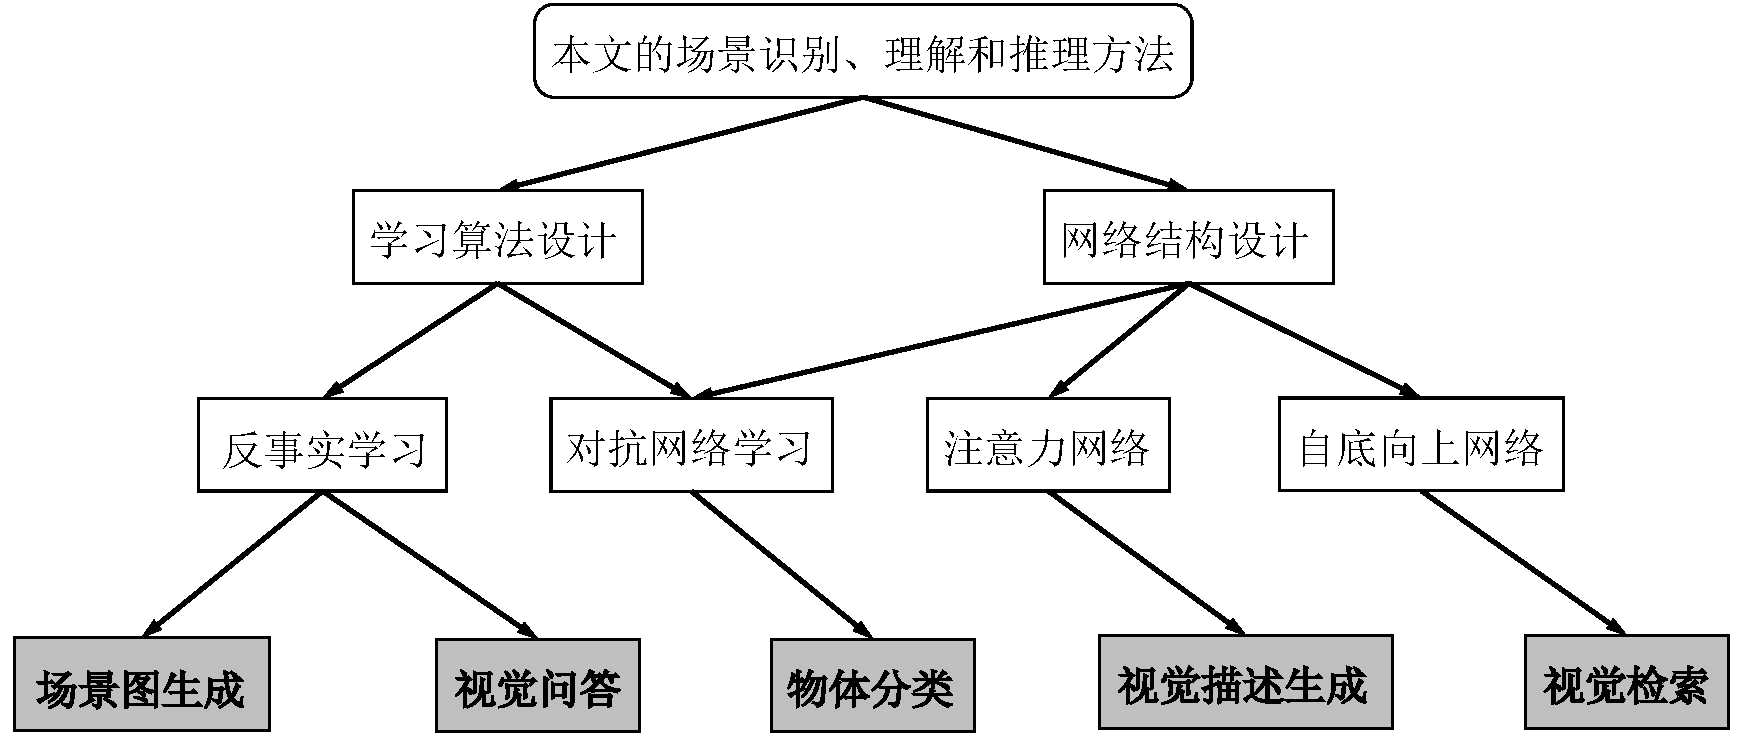
\includegraphics[width=0.95\linewidth]{chapter1/res/technique_summary.pdf}
    \centering
    \caption{复杂场景识别、检测和推理的关键技术研究方法}
    \label{ch1:fig:technique_summary}
\end{figure}

\subsection{基于属性保持对抗网络的零样本物体分类}
复杂视觉场景的感知和理解,其首要步骤就是对视觉场景内的物体进行个体层次的识别。其中本文涉及到的关键技术为零样本物体分类,也称零样本学习。

目前主流的零样本物体分类模型都是基于嵌入映射的框架,这类方法主要是先在训练集上学习一个图像视觉特征与类别属性特征之间的映射函数,然后直接将学习到的映射函数迁移到测试集中。由于训练集和测试集之间的类别存在差异,这些映射函数在测试集中不可避免地存在语义丢失的问题。针对这一普遍问题,本文提出一种全新的零样本学习网络:基于属性保持的对抗网络。该网络通过引入两个独立的映射网络分支,将图像分类和图像重建两个原本相互冲突的任务分离出来。然后利用对抗网络学习让重建网络的特征向量的部分属性能够迁移到分类网络的特征向量中,从而使得分类网络的特征向量能够保持尽可能多的属性,减缓语义丢失的问题。本文提出的零样本学习网络不仅可以逼真地重建回原始图像,同时可以在多个数据集上大幅度地提升零样本分类的准确率。

\subsection{基于反事实多智能体学习的图像场景图生成}
在复杂视觉场景的识别中,除了需要对场景内所有的单个物体进行识别,还需要检测物体间的视觉关系。图像场景图生成任务主要研究如何充分地利用视觉场景内各种视觉元素间的内在联系,实现对整个场景层次的识别。

现有的图像场景图生成方法基本都是将场景内所有的物体和视觉关系分类的交叉熵之和作为模型的优化目标。这个优化目标的本质是认为每个物体分类的损失是相互独立的,即它忽略了不同物体对整体场景图生成质量的不同贡献,容易使模型陷入局部最优解。本文提出了一种全新的训练框架,将图像场景图生成任务转换成一个多智能体协同决策问题,并且直接使用最终的场景图生成质量评价指标(Recall@K)作为模型的优化目标。具体来说,我们将图像中的每个物体看成一个单独的智能体,每个智能体的动作空间是所有可能的物体类别。同时,本文提出了一种全新的反事实基准模型,通过固定其他智能体预测的类别,而反事实地“更改”目标智能体的预测类别,来推测目标智能体预测类别的局部贡献。本文提出的反事实智能体学习框架可以通过提升物体类别的预测准确率,来显著提升整个场景图的生成质量。


\subsection{基于多层空间和通道注意力网络的图像描述生成}

图像描述生成是一种典型的视觉场景理解任务。该任务要求模型在对整个视觉场景进行充分的理解之后,生成自然语句来准确地描述场景内容。

现有的图像描述生成模型都是基于编码器-解码器(encoder-decoder)框架:即利用编码网络(如:卷积神经网络)将图像编码成视觉特征向量,然后利用解码网络(如:递归神经网络)将编码的视觉特征向量解码成自然语句。早期的图像描述生成模型都是只将图像编码成一个固定的视觉特征向量,这大大限制了视觉特征向量的表达能力。之后,部分模型开始引入空间注意力机制,通过在每个单词生成的时刻对不同空间区域的视觉特征赋予不同的权重,进行加权得到不同的视觉特征向量。然而,卷积神经网络的特征图(feature map)除了空间维度外,还包含通道和层级两个维度。在不同的通道和层级下,卷积神经网络的特征图所编码的视觉信息也往往不同。本文提出一种全新的多层空间和通道注意力网络,不仅可以充分地挖掘特征图的三个维度之间的联系,提升了编码网络的表达能力,同时,还可以帮助人们理解在图像描述生成过程中卷积神经网络的特征图的变化过程。


\subsection{基于密集型自底向上网络的视频片段检索}

视频片段检索任务也是一种具有广泛应用价值的视觉场景理解任务。给定一个查询内容(query),视频片段检索任务需要模型在视频中定位出与查询内容相匹配的视频片段。

对于视频片段检索任务,目前的方法都属于自顶向下框架或稀疏型自底向上框架。本文首先分析了现有的视频片段检索的主流框架的优缺点,然后针对稀疏型自底向上模型的设计缺陷,我们提出了一种全新的密集型自底向上框架。具体来说,通过将边界预测问题分解成相关性预测和边界回归两个子问题,可以大大降低视频动作边界定位问题的难度。同时,我们提出一个基于图卷积的特征金字塔层,来增强骨干网络编码能力。该框架大大地提升了自底向上模型的检索准确率。对于多种不同的查询形式(如:自然语句和视频片段等),本文提出的密集型自底向上模型都达到了目前最好的性能。


\subsection{基于反事实样本生成的视觉问答}

视觉场景理解的最终目标就是能够在对整个场景内容完成理解之后进行知识推理。视觉问答是最经典的一种视觉推理任务,给定一个与视觉场景内容相关的问题,模型需要在简单的逻辑推理之后给出问题答案。

尽管近年来已经出现了大量的视觉问答模型,但是这些方法都忽略了一个理想视觉问答模型应当具备的两个重要能力:视觉可解释性和文本敏感性。为了提升视觉问答模型的这两个能力,本文提出了一种全新的反事实样本生成机制。通过人为地遮盖图像中的重要区域或问题中的重要单词,同时更改标准答案,生成大量的反事实样本。通过使用原始训练样本和新生成的反事实样本一起对视觉问答模型进行训练,迫使模型关注反事实样本中被遮盖的重要内容,即让模型在决策时关注到“正确的”视觉区域和单词,提升模型的可解释性和问题敏感性。本文提出的反事实样本生成机制可以无缝地运用到任意的视觉问答模型中,提升模型的鲁棒性和准确率。


\section{本文组织结构}
本文通过对复杂视觉场景理解中视觉内容的识别、检测和推理中的一系列典型问题,提出了多个更加优化的学习算法和更加合理的网络结构。全文共分为八章,后续章节安排如下:

\begin{asparaitem}

\item 第二章介绍了与本文相关的关键技术研究,就零样本物体分类、图像场景图生成、图像描述生成、视频片段检索和视觉问答等几方面的相关工作和本文的关系进行综述。

\item 第三章介绍了基于属性保持对抗网络的零样本物体分类方法。本章首次提出图像分类与图像重建本质上是相互冲突的两个子任务。算法通过引入两个独立的映射网络分支,将图像分类和图像重建两个任务分离出来。然后利用对抗网络学习让重建网络的特征向量的部分属性能够迁移到分类网络的特征向量中,从而使得分类网络的特征向量保持尽可能多的属性,减缓语义丢失的问题。此项工作发表在国际顶级计算机视觉会议CVPR上.

\item 第四章介绍了基于反事实多智能体学习的图像场景图生成方法。本章首次将
图像场景图生成问题转化为一个多智能体协同决策问题,并且直接使用整体的场景图生成质量作为优化目标,避免陷入局部最优解。同时,本章提出一种全新的反事实基准模型,有效地对不同物体的预测类别赋予不同的梯度,显著提升物体类别的预测准确率和整体场景图的生成质量。此项工作发表在国际顶级计算机视觉会议ICCV上。

\item 第五章介绍了基于多层空间和通道注意力网络的图像描述生成方法。本章首次提出通道注意力机制,并认为通道注意力机制本质上也属于一种特殊的语义注意力机制。同时,本章提出一种全新的多层空间和通道注意力网络,不仅充分挖掘了卷积神经网络的特征图的三个维度(空间、通道和层级)之间的联系,提升了编码网络的表达能力。同时,还可以帮助人们理解在图像描述生成过程中卷积神经网络的特征图的变化过程。此项工作发表在国际顶级计算机视觉会议CVPR上。

\item 第六章介绍了基于密集型自底向上网络的视频片段检索方法。本章首次提出了一种密集型自底向上网络框架。通过将边界预测问题分解成相关性预测和边界回归两个子问题,大大降低了模型对视频动作边界定位的难度。同时,本章提出了一个基于图卷积的特征金字塔层,来增强骨干网络编码能力。该框架显著地提升了视频片段检索的准确率。此项工作发表在国际顶级人工智能会议AAAI上。

\item 第七章介绍了基于反事实样本生成的视觉问答方法。本章首次提出了一种通用的反事实训练样本生成方法,提升视觉问答模型的视觉可解释性和文本敏感性。本文提出的反事实样本生成机制可以无缝地运用到任意的视觉问答模型中,提升模型的准确率和鲁棒性。此项工作发表在国际顶级计算机视觉会议CVPR上。

\item 第八章对全文介绍的工作进行了总结,并提出了对进一步对复杂场景理解的识别、检测和推理的研究内容以及今后的研究展望。

\end{asparaitem}

\section{本章小结}
本章对复杂视觉场景的识别、检测和推理问题进行了叙述,分别介绍了研究背景、本文的主要研究内容以及全文的组织结构。

